\documentclass[a4paper, 12pt, oneside]{extarticle}
%-shell-escape % якщо використовуєте minted
\input{$HOME/Templates/lpnu_doc_templates/settings/preamble.tex}
% якщо домахуються дуже за Times New Roman, то
% використовуєте xelatex і цей файл:
\input{$HOME/Templates/lpnu_doc_templates/settings/minted_settings.tex}

\newcommand\Variant{4}
\newcommand\Date{14.04.\the\year}
\newcommand\Discipline{Об'єктно-орієнтоване програмування}
\newcommand\Instructor{Патерега Ю. І.}

\newcommand\Type{\Lab}
\newcommand\Number{3}
\newcommand\Topic{Перевантаження операцій. Файлові потоки даних}
\setcounter{secnumdepth}{0}

\begin{document}
\Margins

\Margins
%\begin{wrapfigure}[3]{l}{.27\textwidth}
%\includegraphics[width=.28\textwidth]{$UNI/.templates/lpnu_logo.png}
%\end{wrapfigure}

%\noindent\textbf{Прізвище:} \Lname \\
%\noindent\textbf{Ім'я:} \Fname \\
%\noindent\textbf{Група:} \Group \\
%\noindent\textbf{Варіант:} \Variant \\
%\noindent\textbf{Дата захисту:} \Date \\
%\\
%\noindent\textbf{Кафедра:} \Department \\
%\noindent\textbf{Дисципліна:} \Discipline \\
%\noindent\textbf{Перевірив:} \Instructor \\

%%\medskip\bigskip

%\begin{center}
%	\textbf{ЗВІТ}		\\
%	до \Type~\No\Number	\\
%	на тему ``\Topic''	\\
%\end{center}

% \begin{table}
%   \begin{tabularx}{\textwidth}{|c|X|X|}
%     \hline
%     % Image & Content & Additional Info \\
%     % \hline
% 	  \multirow{3}{*}{\includegraphics[width=4cm]{$UNI/.templates/lpnu_logo.png}}
% 	  & \textbf{ЗВО:}
% 	  Національний університет ``Львівська Політехніка''.
% 	  & \textbf{Тема:}
% 	  \Topic
% 	  \\
% 	  & \textbf{Навчальний рік:}
% 	  2023/2024
% 	  & \textbf{Інститут}
% 	  комп'ютерних наук та інформаційних технологій
% 	  \\
% 	  & \textbf{Семестр:}
% 	  осінній
% 	  & \textbf{Група:}
% 	  \Group
% 	  \\
% 	  & \textbf{Навчальна дисципліна:}
% 	  \Discipline
% 	  & \textbf{Студент:}
% 	  Мілюхін Олександр
% 	  \\
% 	  & \textbf{Кафедра}
% 	  систем автоматизованого проектування
% 	  &
% 	  \\
% 	  & \textbf{Викладач:}
% 	  Чумакевич В. В.
% 	  &
% 	  \\
%     \hline
%   \end{tabularx}
% \end{table}

\setlength{\textfloatsep}{-16pt}
% \setlength{\intextsep}{0pt}

\begin{table}
	\begin{tabular}{|l|l|p{6cm}|}
    \hline
    % Image & Content & Additional Info \\
    % \hline
	  \makecell[l]{
	  \includegraphics[width=3.37cm]{$UNI/.templates/lpnu_logo.png}
  }
	  & \makecell[l]{
	  \textbf{ЗВО:}
	  Національний університет \\ ``Львівська Політехніка''.
	  \\
	  \textbf{Навчальний рік:}
	  2023/2024
	  \\
	  \textbf{Семестр:}
	  осінній
	  \\
	  \textbf{Навчальна дисципліна:} \\
	  \Discipline
	  \\
	  \textbf{Кафедра}
	  систем автоматизованого \\ проектування
	  \\
	  \textbf{Викладач:}
	  Чумакевич В. В.
}
	  & \makecell [l] {
	  \textbf{Тема:}
	  \Topic
	  \\
          \textbf{Інститут}
	  комп'ютерних наук та \\ інформаційних технологій
	  \\
	  \textbf{Група:}
	  \Group
	  \\
	  \textbf{Студент:}
	  Мілюхін Олександр
  }
  \\
    \hline
  \end{tabular}
\end{table}
\section{Мета роботи}

% \begin{table}
%   \begin{tabularx}{\textwidth}{|p{6cm}|c|c|}
% 	  \hline
%     \multirow{3}{*}{\includegraphics[width=6cm]{$UNI/.templates/lpnu_logo.png}}
% 	  & ЗВО: Національний університет ``Львівська Політехніка''
% 	  & Additional Info 1 \\
%     & Content 2 & Additional Info 2 \\
%     & Content 3 & Additional Info 3 \\
% 	  \hline
%   \end{tabularx}
% \end{table}

% \begin{table}
%   \begin{tabular}{|c|c|c|}
%     \hline
%     \multirow{3}{*}{\includegraphics[width=3cm]{$UNI/.templates/lpnu_logo.png}} & \makecell{Content 1 \\ Content 2 \\ Content 3} & \makecell{Additional Info 1 \\ Additional Info 2 \\ Additional Info 3} \\
%     \hline
%   \end{tabular}
% \end{table}


Навчитись перевантажувати операції зчитування та запису, а також
арифметичні операції для створених об’єктів.

\section*{Індивідуальне завдання}

\subsection*{Завдання 1}

Описати клас, що реалізовує вказаний нижче тип даних. Клас повинен
містити конструктор та подані нижче операції над об’єктами (плюс обов’язково
операції порівняння та присвоєння) з використанням перевантаження операцій.
Написати програму, яка демонструє роботу з об’єктами цього класу.
Програма повинна містити меню для перевірки усіх методів цього класу і
операцій.

\paragraph{4.}
Вектор у площині Віднімання та складання векторів

\subsection*{Завдання 2}

Виконати завдання, подані в таблиці з використанням файлових потоків і
методів обробки помилок.
Вхідні дані необхідно прочитати з файла \texttt{file\_input.txt}, а всі результати
роботи програми вивести на екран і записати у файл \texttt{file\_output.txt.}

\paragraph{4}
Написати програму, яка копіює вміст вхідного файла у вихідний; перевіряє, чи
співпадає кількість відкритих і закритих дужок у введеному рядку (перевірити для
круглих та квадратних дужок); знаходить найдовше слово; видаляє всі слова, що
складаються тільки з латинських літер

\section*{Етапи розв'язку}

\subsection*{Код програми (завдання 1)}

\inputminted{c++}{task1/main.cpp}
\inputminted{c++}{task1/vector.h}
\inputminted{c++}{task1/vector.cpp}
\inputminted{c++}{task1/makefile}

\subsection*{Результат виконання програми}

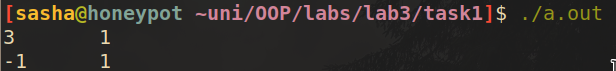
\includegraphics[width=.7\textwidth]{bruh.png}

\subsection*{Код програми (завдання 2)}

\subsubsection{main.cpp}
\inputminted{c++}{task2/src/main.cpp}
\subsubsection{file_manager.cpp}
\inputminted{c++}{task2/src/file_manager.cpp}
\subsubsection{text_manager.cpp}
\inputminted{c++}{task2/src/text_manager.cpp}
\subsubsection{file_manager.h}
\inputminted{c++}{task2/include/file_manager.h}
\subsubsection{text_manager.h}
\inputminted{c++}{task2/include/text_manager.h}
\subsubsection{Makefile}
\inputminted{make}{task2/src/Makefile}

\subsection*{Вміст file_input.txt}

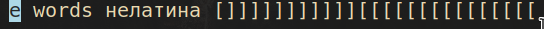
\includegraphics[width=.5\textwidth]{/home/sasha/Documents/uni/2-сем/OOP/labs/lab3/pic-selected-230414-1207-26.png}

\subsection*{Результат виконання програми}

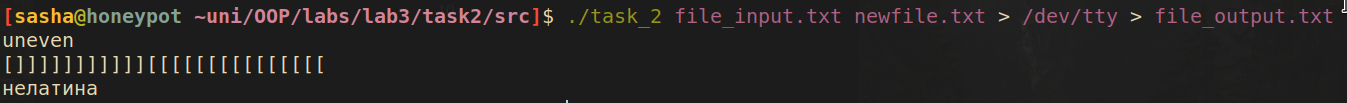
\includegraphics[width=\textwidth]{/home/sasha/Documents/uni/2-сем/OOP/labs/lab3/task2/src/out.png}

\subsection*{Вміст file_output.txt}
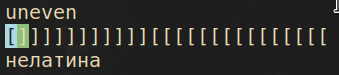
\includegraphics[width=.3\textwidth]{/home/sasha/Documents/uni/2-сем/OOP/labs/lab3/task2/src/img/pic-selected-230414-1151-58.png}

\subsection*{\texttt{newfile.txt}}

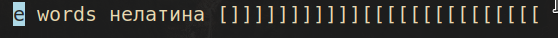
\includegraphics[width=.5\textwidth]{/home/sasha/Documents/uni/2-сем/OOP/labs/lab3/pic-selected-230414-1208-12.png}

\subsection{file_input з однаковою кількістю дужок}

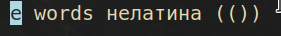
\includegraphics[width=.3\textwidth]{/home/sasha/Documents/uni/2-сем/OOP/labs/lab3/task2/src/img/pic-selected-230414-1151-27.png}

\subsection*{Результат виконання програми з однаковою кількістю відкритих/закритих дужок у file_input.txt}

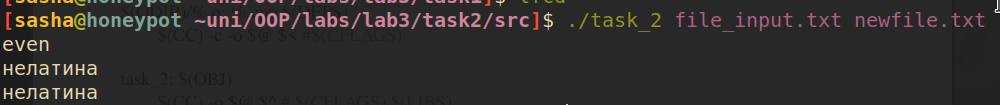
\includegraphics[width=.9\textwidth]{un.png}

\subsection*{\texttt{newfile.txt}}

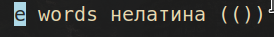
\includegraphics[width=.3\textwidth]{/home/sasha/Documents/uni/2-сем/OOP/labs/lab3/task2/src/img/pic-selected-230414-1152-43.png}

\subsection{file_output.txt}

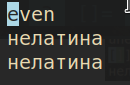
\includegraphics[width=.2\textwidth]{/home/sasha/Documents/uni/2-сем/OOP/labs/lab3/pic-selected-230414-1227-36.png}

\section*{Висновок}

Ознайомився з перевантаженням операцій та роботою з файлами засобами
мови C++. Реалізував перевантажені бінарні оператори для векторів і
програму-аналізатор текстових файлів.

\section*{Відповіді на контрольні запитання}
\begin{itemize}
	\question	Який загальний синтаксис перевантаження операцій?
	\answer
	\begin{verbatim}
	тип_значення operator знак_операції (Список параметрів
	перевантаженої операції).
	{
	оператори
	}
	\end{verbatim}

	\question	Для чого використовується перевантаження операцій?
	\answer Для спрощення запису та інтуїтивного сприйняття дій з об'єктами класів.
	\question	Які операції не можна перевантажити у С++?
	\answer Не можна перевантажувати ”.”, ”::”, ”,”, ”.*”, ”?:”, sizeof, typeid, static_cast ,dynamic_cast, const_cast.
	\question	Назвіть правила перевантаження операцій у С++?
	\answer Не можна змінювати базовий функціонал оператора, кількість його аргументів та пріоритет.
	\question	Коли необхідно перевантажувати операцію присвоєння?
	\answer Коли треба створити клас, що має
	\question	Як передаються параметри під час перевантаження операції?
	\answer Так само, як і до функцій (методів класу).
	\question	Що таке файлові потоки даних? Наведіть приклад.
	\answer Файлові потоки даних - це механізм вводу та виводу даних, який дозволяє програмі взаємодіяти зі збереженими на диску файлами як зі стандартними потоками вводу та виводу. Наприклад, у C++ для цього є класи fstream, ifstream, та інші.
\end{itemize}

\end{document}
